%%%%%%%%%%%%%%%%%%%%%%%%%%%%%%%%%%%%%%%%%%%%%%%%%%%%%%%%%%%%%%%%%%%%%%%%%%
% Output voltage u2 for M3C with RL-Load
%%%%%%%%%%%%%%%%%%%%%%%%%%%%%%%%%%%%%%%%%%%%%%%%%%%%%%%%%%%%%%%%%%%%%%%%%%
\begin{solutionfigure}[htb]

    %   \documentclass{standalone}
    %   \usepackage{pgfplots}
    %   \pgfplotsset{compat=1.18} % Kompatibilität für neuere Versionen
           \centering
           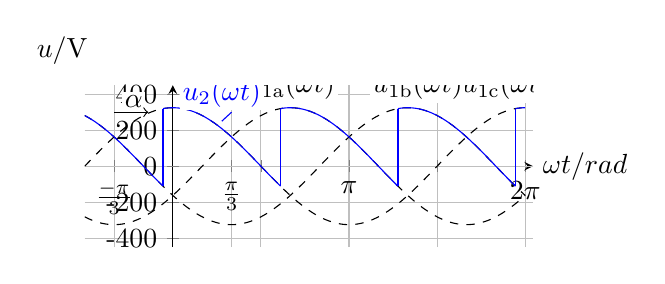
\begin{tikzpicture}
               \begin{axis}[
                   % x/y range adjustment
                   xmin=-90, xmax=368,
                   ymin=-450, ymax=450,
                   samples=500,
                   axis y line=center,
                   axis x line=middle,
                   extra y ticks=0,
                   % Label text
                   xlabel={$\omega t / \text{rad}$},,
                   ylabel={$u/\mathrm{V}$},
                   % Label adjustment
                   x label style={at={(axis description cs:1,0.5)},anchor=west},
                   y label style={at={(axis description cs:-.05,.97)},anchor=south,yshift=0.2cm},
                   width=0.6\textwidth,
                   height=0.3\textwidth,
                   % x-Ticks
                   xtick={-60,0,60,90,180,270,360},
                   xticklabels={$\frac{-\pi}{3}$,,$\frac{\pi}{3}$,,$\pi$,,$2\pi$},
                   xticklabel style = {anchor=north},
                   % y-Ticks
                   ytick={400,200,0,-200,-400},
                   yticklabels={400,200,0,-200,-400},
                   yticklabel style = {anchor=east},
                   % Grid layout
                   grid,
                   %grid style={line width=.1pt, draw=gray!10},
                   %major grid style={line width=.2pt,draw=gray!90},
               ]
               % Voltage u1a(wt), u1b(wt) u1c(wt)
               \addplot[black, domain= -90:360,dashed] {325*cos(x)};                
               \addplot[black, domain= -90:360,dashed] {325*cos(x+120)};                
               \addplot[black, domain= -90:360,dashed] {325*cos(x+240)}; 
               % Voltage u2(wt)
               \addplot[blue, domain= -90:-10] {325*cos(x+120)}; 
               \addplot[blue, domain= -10:110] {325*cos(x)};                
               \addplot[blue, domain= 110:230] {325*cos(x+240)};                
               \addplot[blue, domain= 230:350] {325*cos(x+120)};
               \addplot[blue, domain= 350:360] {325*cos(x)}; 
               \addplot[color=blue,solid] coordinates{
                (-10,-111)
                (-10, 317)
            };               
               \addplot[color=blue,solid] coordinates{
                   (110,-111)
                   (110, 317)
               };     
               \addplot[color=blue,solid] coordinates{
                   (230,-111)
                   (230, 317)
               };     
               \addplot[color=blue,solid] coordinates{
                   (350,-111)
                   (350, 317)
               };
        
               % Label of u1c
               \node[black, fill=white, inner sep = 1pt, anchor = south] at (axis cs:340,350) {$u_{\mathrm{1c}}(\omega t)$}; 
               % Label of u1a
               \node[black, fill=white, inner sep = 1pt, anchor = south] at (axis cs:120,350) {$u_{\mathrm{1a}}(\omega t)$};           
               % Label of u1b
               \node[black, fill=white, inner sep = 1pt, anchor = south] at (axis cs:250,350) {$u_{\mathrm{1b}}(\omega t)$};
               % Label of u2
               \node[blue, fill=white, inner sep = 1pt, anchor = south] at (axis cs:50,310) {$u_{\mathrm{2}}(\omega t)$};
               %Label Firing angle 
               \node[black, fill=white, inner sep = 1pt, anchor = south] at (axis cs:-40,310){$\alpha$};
               % Line to u2
               \draw[thin, blue] (60,300) -- (50,250);
               \draw[->](-60,300) -- (-25,300); 
           \end{axis}     
           \end{tikzpicture}
           \caption{Output voltage $u_\mathrm{2}(t)$ for $\alpha = 0.871$.}
           \label{sfig:ex06_output_voltage_6_1_3}
   \end{solutionfigure}